\documentclass{db-practice}

\begin{document}

\title{Ejercicio de índices}

\section*{Ejercicio de índices}

Los índices en una base de datos son estructuras de datos orientadas a mejorar la velocidad de las operaciones. Se forman mediante identificadores únicos para una tabla de la base de datos y permiten un acceso más rápido a los registros, evitando tener que realizar en las consultas la lectura secuencial de todas las filas que componen una tabla \textit{(Full Table Scan)}. 

No obstante, si no sabemos utilizar correctamente un índice podemos acrecentar su mayor inconveniente. Y es que ocurre, que cuando creamos un índice sobre una tabla y queremos modificar esa tabla después (\texttt{INSERT, DELETE, UPDATE}), todos los índices asociados a esta tabla también se modificarán. Es decir, se ralentizan las operaciones de escritura sobre las tablas que tengan índices. 

A continuación, vamos a trabajar con la creación y la utilización de índices dentro de nuestra base de datos, a fin de poder comprobar el funcionamiento del sistema en MySQL. Para ello, sigue las instrucciones que aparecen a continuación, manteniendo el orden de las mismas y presta atención al comportamiento de las operaciones. 

\subsection*{Creación de índices}

Como primer paso hacia las creaciones de índices, debemos entender que sin darnos cuenta cuando creábamos claves primarias en una tabla, ya estábamos creando un índice asociado a esa clave primaria de forma automática. No obstante, si queremos forzar la creación de un índice podemos hacerlo de tres maneras diferentes: 

\begin{enumerate}
    \item Podemos crear el índice directamente: 
    \begin{lstlisting}[language=SQL]
CREATE INDEX indice ON tabla (columna); 
    \end{lstlisting}
        
    \item Modificando una tabla ya creada: 
    \begin{lstlisting}[language=SQL]
ALTER TABLE tabla ADD INDEX (columna1, [columna2, ...]); 
    \end{lstlisting} 

     \item En la misma creación de la tabla: 
     \begin{lstlisting}[language=SQL]
CREATE TABLE tabla (columna VARCHAR(32), INDEX(columna)); 
     \end{lstlisting} 
\end{enumerate}

\subsection*{Consideraciones de MySQL Workbench}

MySQL Workbench es una herramienta muy completa que nos permite trabajar de una manera analítica sobre nuestra base de datos. Una de sus funcionalidades nos permite conocer el coste computacional de nuestras consultas. Para hacer uso de ella, simplemente a la hora de ejecutar una consulta deberemos usar el icono del rayo con una lupa (ver Figura \ref{fig:mysqlwork}). 

\begin{figure}[ht]
    \centering
    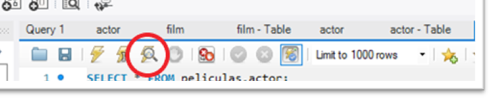
\includegraphics[width=0.5\columnwidth]{figs/mysqlwork-analysis.png}
    \caption{Opción de \emph{explain} para ejecuciones analíticas.}\label{fig:mysqlwork}
\end{figure}

Al ejecutar una consulta con esta opción, MySQL Workbench nos mostrará una pestaña adicional (\emph{explain}) que contiene información sobre el coste de nuestras consultas, así como también nos aporta información del tipo de búsqueda que se ha llevado a cabo en cada operación.

\begin{figure}[ht]
    \centering
    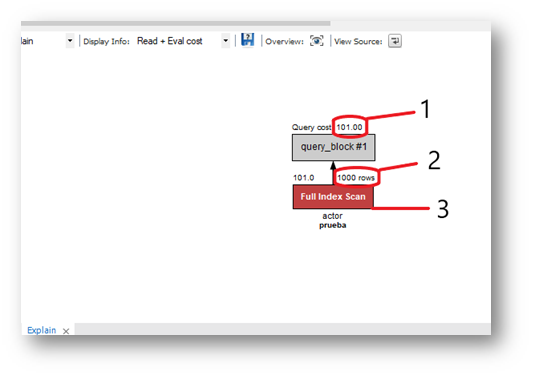
\includegraphics[width=0.8\columnwidth]{figs/example.png}
    \caption{Ejemplo resultado ejecución de \emph{explain}.}\label{fig:example}
\end{figure}

Al ejecutar una consulta sencilla con esta opción de ejecución, podemos recopilar mucha información de cómo trabaja nuestro gestor de bases de datos. Para ello vamos a analizar un resultado cualquiera como el que se muestra en la Figura \ref{fig:example}:

\begin{enumerate}
    \item \textbf{Query Cost}: el coste computacional de esta consulta que es de 101.00.  Este parámetro es calculado en base a unas estadísticas que el gestor de la base de datos mantiene en todo momento y que puede reiniciar cuando el administrador lo desea. Esto quiere decir, que una misma consulta puede arrojar valores diferentes dependiendo del ordenador en donde se realice. 
    \item \textbf{Rows}: el número de filas que devuelve la consulta. Este valor se tiene en consideración sobre todo en consultas más complejas para poder llevar un registro más minucioso.
    \item \textbf{Tipo de búsqueda}: en este caso, el resultado obtenido es una lectura secuencial completa y a pesar de que ha utilizado un índice, la consulta ha tenido que recorrer todas las filas de que dispone la tabla. Este punto es especialmente interesante ya que nos permite conocer de forma intuitiva en que sitios necesitamos crear un índice para agilizar las consultas.
\end{enumerate}

\subsection*{Consultas y resultados de ejecución}

Para entrar más en detalle, sobre la base de datos vamos a realizar una consulta que podamos optimizar y de esta manera podremos seguir el proceso completo y analizar el verdadero impacto que tienen los índices respecto de la eficiencia de las consultas.

\subsubsection*{Preparación de los datos}

Carga el fichero \texttt{peliculas.sql} que puedes encontrar en el Moodle de la asignatura.

\subsubsection*{Consulta}

Crea la consulta que muestre el nombre y apellidos del actor ``Lonzo Bode'', así como el número total de películas en las que ha participado.
    
\begin{lstlisting}[language=SQL]
SELECT ac.first_name, ac.last_name, COUNT(*) Total
FROM (SELECT fi.film_id, actor_id 
      FROM film fi 
        INNER JOIN film_actor fiac 
            ON fi.film_id = fiac.film_id) jo 
        INNER JOIN actor ac 
            ON ac.actor_id=jo.actor_id
WHERE ac.first_name="Lonzo" AND ac.last_name="Bode"
GROUP BY ac.first_name, ac.last_name;
\end{lstlisting} 

Si ejecutamos la consulta y miramos su \emph{explain} podemos apreciar diferentes aspectos a tener en cuenta sobre la misma consulta de la Figura \ref{fig:ejecucion1}.

\begin{figure}[ht]
    \centering
    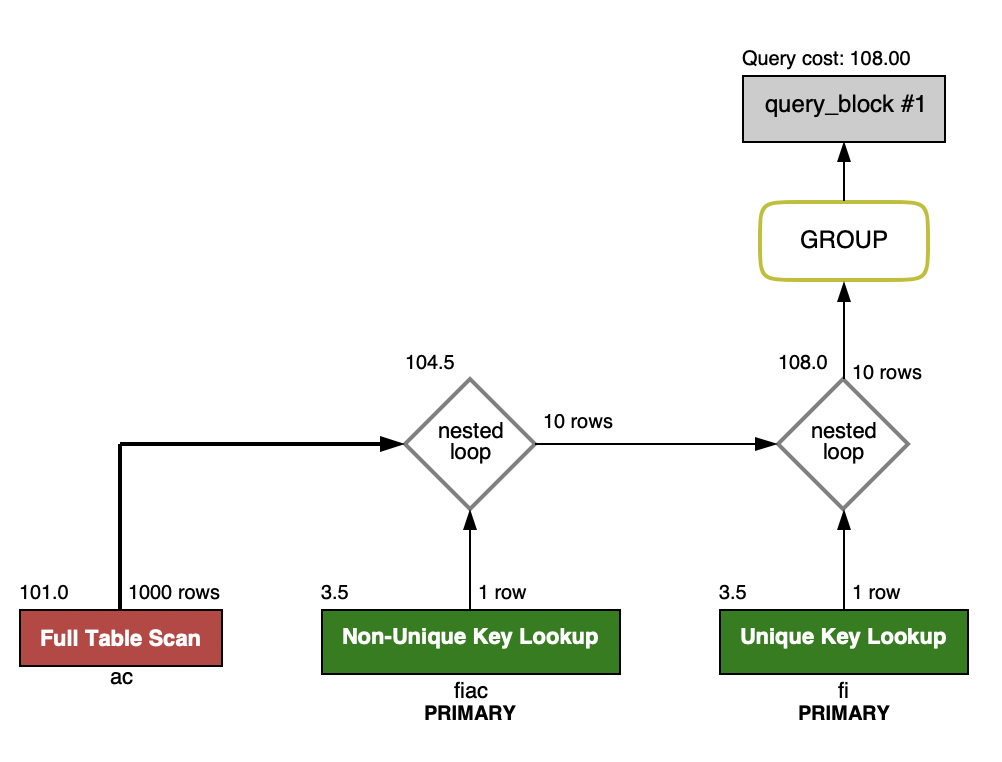
\includegraphics[width=0.8\columnwidth]{figs/ejecucion1.png}
    \caption{Resultado del \emph{explain} al ejecutar la consulta.}\label{fig:ejecucion1}
\end{figure}

\begin{itemize}
    \item A pesar de que aún no hemos realizado ninguna operación de modificación sobre la base de datos, las dos cajas verdes nos dan mucha información de los índices primarios asociados a las claves primarias de cada tabla. Y es que estas dos cajas son el resultado de la búsqueda por clave repetida (\emph{Non-Unique Key Lookup}) y por clave única respectivamente (\emph{Unique Key Lookup}). Y es debido a que nuestra base de datos ha usado estos índices que el coste es tan bajo.
    \item No obstante, la diferencia entre usar índices y no usarlos se ve reflejado en la caja roja. Si nos fijamos en el coste computacional de la segunda parte de la consulta se aprecia que en torno al 90\% del tiempo que tarda esta consulta reside en esta parte. La conclusión es sencilla, la base de datos se ha visto obligada a realizar una lectura completa de la tabla para encontrar a ``Lonzo Bode''.
    \item Si nos fijamos aún más en el resultado podemos interpretar cómo ha realizado los \texttt{JOIN} de cada una de las tablas. El primer \texttt{JOIN}, lo ha ejecutado sobre la tabla \texttt{actor} y la tabla \texttt{film-actor}. El resultado devuelve 20 filas que se muestra en el primer rombo de \emph{nested loop}. Por tanto, en el segundo rombo tendremos el resultado del segundo  \texttt{JOIN} con la tabla \texttt{film}.
\end{itemize}

\subsubsection*{Optimización}

Ahora que ya hemos visto cómo funcionan los índices primarios y la diferencia de tiempo que existe al realizar una consulta sin índices, vamos a tratar de crear nuestro propio índice para mejorar la eficiencia de la consulta. Lo primero que tenemos que fijarnos es que la consulta buscaba a ``Lonzo'' por dos campos, ``first\_name'' y ``last\_name'', por tanto, si queremos realizar un índice que se use para esta consulta, tiene que ser un índice compuesto que contenga los dos campos.

\begin{lstlisting}[language=SQL]
ALTER TABLE actor
ADD INDEX optimizar (first_name ASC, last_name ASC) VISIBLE;
\end{lstlisting}

Con la sentencia anterior crearemos el índice compuesto que nos permitirá optimizar la consulta. Una vez lo creemos, deberemos volver a ejecutar la consulta para ver los resultados.

\begin{figure}[ht]
    \centering
    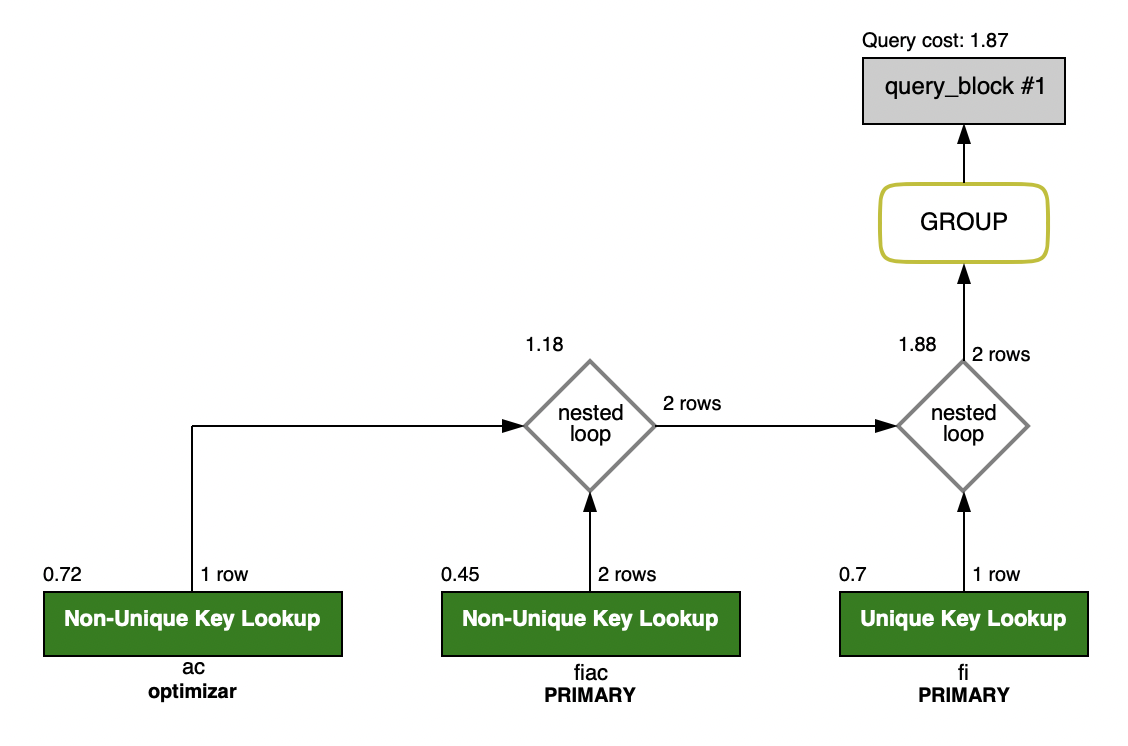
\includegraphics[width=0.8\columnwidth]{figs/ejecucion1optimizada.png}
    \caption{Resultado del explain al ejecutar la consulta optimizada.}\label{fig:ejecucion1optimizada}
\end{figure}

Una vez ejecutada la consulta (ver Figura \ref{fig:ejecucion1optimizada}, se puede apreciar que hemos mejorado la consulta fijándonos directamente en el coste, y es que hemos pasado de $108.00 \rightarrow 1.87$. Además del coste, podemos apreciar que índice se ha utilizado para corroborar que todo haya ido bien. Si nos fijamos debajo de nuestra caja asociada a la consulta debe aparecer el nombre que le hemos dado a nuestro índice, en este caso ``optimizar'' (ver Figura \ref{fig:ejecucion1part1}).

\begin{figure}[ht]
    \centering
    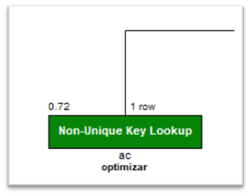
\includegraphics[width=0.3\columnwidth]{figs/ejecucion1part1.png}
    \caption{Resultado del \emph{explain} al ejecutar la consulta optimizada primera subconsulta.}\label{fig:ejecucion1part1}
\end{figure}

Ahora que ya creemos haber optimizado al completo nuestra consulta, vamos a tratar de crear un índice más simple para nuestra consulta para ver como trabaja nuestra base de datos. Para ello, creamos un índice que solo contenga ``first\_name'':

\begin{lstlisting}[language=SQL]
ALTER TABLE actor
ADD INDEX optimizar (first_name ASC) VISIBLE;
\end{lstlisting}

Y una vez creado ejecutamos de nuevo nuestra consulta. Si todo ha funcionado correctamente nos daremos cuenta de que el gestor ha decido utilizar este índice y no el anterior, obteniendo incluso mejores resultados a pesar de devolver 2 filas en la sentencia (ver Figura \ref{fig:ejecucion1coste}).

\begin{figure}[ht]
    \centering
    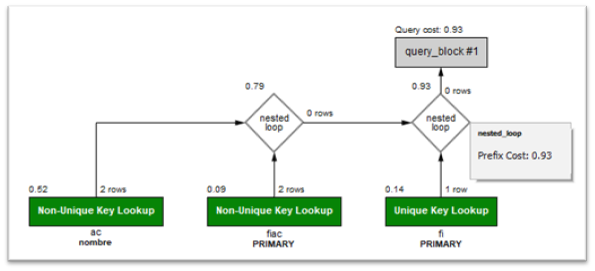
\includegraphics[width=0.6\columnwidth]{figs/ejecucion1coste.png}
    \caption{Coste computacional de una sección de la consulta.}\label{fig:ejecucion1coste}
\end{figure}

\subsubsection*{Desventajas}

Para finalizar, hemos de tener muy claro que los índices no solo nos permiten optimizar y agilizar nuestras consultas, sino que pueden afectar muy negativamente las escrituras en la base de datos. Como se ha mencionado al principio, al crear un índice sobre una tabla, para cualquier modificación de la tabla también se actualizará los índices asociados y por ello costará más tiempo llevar las operaciones a cabo.

\begin{figure}[ht]
    \centering
    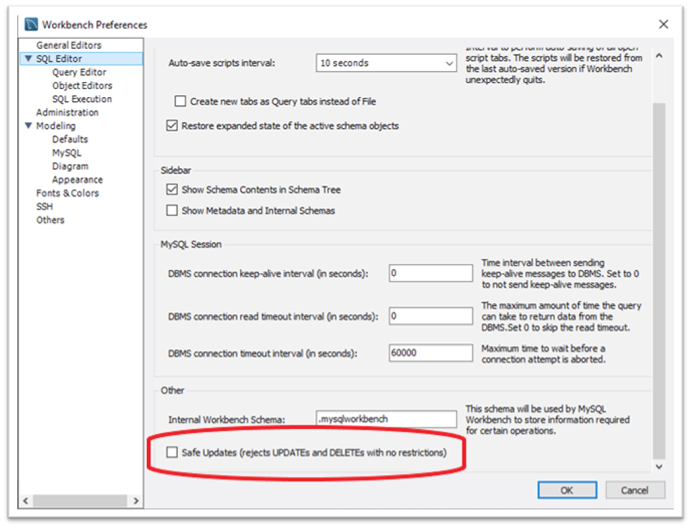
\includegraphics[width=0.6\columnwidth]{figs/WorkbenchPreferences.png}
    \caption{Ventana de preferencias de MySQL Workbench.}\label{fig:preferences}
\end{figure}

Para poner a prueba esta cualidad, vamos a preparar una escritura en la tabla \texttt{film}. No obstante, para poder llevar a cabo la operación antes tenemos que desactivar la opción de \emph{safe update} de nuestro MySQL Workbench. Para acceder a esta opción (ver Figura \ref{fig:preferences}) seguimos la siguiente ruta: Edit $\rightarrow$ Preferences.

Ahora vamos a realizar la operación de escritura, para ello queremos actualizar la duración de las películas e incrementar en uno todas aquellas que duran mas de 100 minutos, para ello utilizamos la siguiente consulta:

\newpage

\begin{lstlisting}[language=SQL]
UPDATE film
SET length_minutes = length_minutes +1 
WHERE length_minutes >= 100;
\end{lstlisting}

Antes de ejecutar nuestra consulta debemos tener en cuenta que esta operación la queremos realizar repetidas veces sobre nuestra tabla para comprobar las diferencias, y para ello tenemos que fijarnos en la duración de la consulta tal y como indica la Figura \ref{fig:tiempoEjecucion}. Este valor diferirá dependiendo de la maquina en que ejecutemos nuestra consulta, pero podemos tomarlo como referencia. Una vez realizada la consulta es momento de trastear creando índices que incluyan la columna ``length\_minutes''. Podemos crear la cantidad de índices que queramos, a cuantos más creemos mayor será la diferencia. 

\begin{figure}[ht]
    \centering
    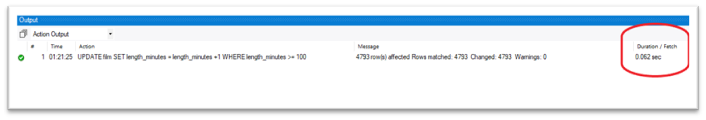
\includegraphics[width=0.9\columnwidth]{figs/tiempoEjecucion.png}
    \caption{Tiempo de computación para cada ejecución.}\label{fig:tiempoEjecucion}
\end{figure}

Cuando terminemos de crear índices, ejecutamos otra vez la sentencia y comparamos los resultados.

\end{document}